\documentclass{elegantbook}

\author{ddswhu \& Liam Huang}
\email{ddswhu@outlook.com}

\zhtitle{优美的 \LaTeX{} 书籍}
\zhend{模板}
\entitle{Elegant\LaTeX{} Book}
\enend{Template}
\version{3.03}
\myquote{Victory won\rq t come to us unless we go to it.}
\logo{ElegantLaTeX_green.pdf}
\cover{cover.pdf}

%green color
   \definecolor{main1}{RGB}{0,120,2}
   \definecolor{second1}{RGB}{230,90,7}
   \definecolor{third1}{RGB}{0,160,152}
%cyan color
   \definecolor{main2}{RGB}{0,175,152}
   \definecolor{second2}{RGB}{239,126,30}
   \definecolor{third2}{RGB}{120,8,13}
%blue color
   \definecolor{main3}{RGB}{20,50,104}
   \definecolor{second3}{RGB}{180,50,131}
   \definecolor{third3}{RGB}{7,127,128}

\usepackage{makecell}
\usepackage{lipsum}
\usepackage{texnames}

\begin{document}
\maketitle
\tableofcontents
\mainmatter
\chapter{Elegant\LaTeX{} 系列模板介绍}

值此版本发行之际,我们 Elegant\LaTeX{} 项目组向大家重新介绍一下我们的工作,我们致力于打造一系列美观、优雅、简便的模板方便用户使用。Elegant\LaTeX{} 系列模板目前由 ElegantNote,ElegantBook,ElegantPaper,ElegantBeamer 组成,分别用于排版笔记,书籍,工作论文和幻灯片讲稿。这些子项目的名词是一体的,请在使用这些名词的时候不要将其断开(如 Elegant Note 是不正确的写法)。并且,Elegant\LaTeX{}  Book 指的即是 ElegantBook。

请用户在作者的主页下载最新版本,下载地址:\href{https://ddswhu.me/resource/}{https://ddswhu.me/resource/}。本文将介绍本模板的一些设置内容以及基本使用方法。如果您在使用此模板,欢迎把您使用此模板制作的成品发一份给我们,谢谢!如果您有其他问题,建议或者意见,欢迎联系我:\mailto{ddswhu@outlook.com}。


\section{ElegantBook 更新说明}
在这几年间,我们收到了很多用户的反馈,主要的问题涉及到字体安装,编码支持,定理浮动,定理跨页,交叉引用等等。我们思前想后,原先让用户安装字体以追求视觉上的美观并不完美,用户陷入了巨大的麻烦,这违背了我们的模板初衷。因此我们在新版中删除了这部分,用户无需安装任何字体。让我们来看下此次 ElegantBook 模板 3.0 更新的主要内容有:

\begin{enumerate}[noitemsep]
   \item 删除了自定义字体设置,改用 \texttt{ctex} 宏包用以支持中文。
   \item 使用 \texttt{tcolorbox} 宏包改写了原先的定理类环境,目前定理环境等均可以跨页。
   \item 重新命名了定理类环境的名称(theorem,definition,proposition 等)。
   \item 重新命名了颜色的名字(first,second,third)。
\end{enumerate}

\section{未来更新计划}


\begin{enumerate}[noitemsep]
   \item 设计一个适合的 LOGO;
   \item 重新设计 base 图标;
   \item 重新设计一个好看的封面。
   \item 将基础模板改为英文模板,添加选项使其支持中文。
   \item 将最早的 ElegantNote 重新设计为简版发布。
   \item 添加一个简化风格(plain)的颜色主题。
\end{enumerate}

\chapter{ElegantBook 设置说明}


\section{编译方式}

本模板基于基础的 book 文类,所以 book 的选项对于本模板也是有效的。默认编码为 UTF-8,推荐使用 \TeX{} Live 编译。作者编写环境为 Win10(64bit) + \TeX{} Live 2018。由于使用的是 \texttt{ctex} 宏包,所以支持 \texttt{pdflatex} 以及 \texttt{xelatex} 编译。


\section{选项设置}
本文特殊选项设置共有 2 类,分为 {\color{main}主题颜色}设置 以及 {\color{main}章标题显示风格}设置。

第 1 类为{\color{main}主题颜色}设置,内置 3 组颜色主题,分别为 \verb|green|(默认)、\verb|cyan|、\verb|blue|,另外还有一个自定义的选项  \verb|nocolor|。调用颜色主题 \verb|green| 的方法为 \\
\verb|\documentclass[green]{elegantbook}| 或者 \verb|\documentclass[color=green]{elegantbook}|。需要改变颜色的话请选择 \verb|nocolor| 选项或者使用 \verb|color=none|,然后在导言区定义 main、second、third 颜色,具体的方法如下:

\begin{verbatim}
\definecolor{main}{RGB}{70,70,70}    %定义 main 颜色值
\definecolor{second}{RGB}{115,45,2}    %定义 second 颜色值
\definecolor{third}{RGB}{0,80,80}     %定义 third 颜色值
\end{verbatim}

\begin{table}[htp]
\caption{ElegantBook 模板中的三套颜色主题\label{tab:color thm}}
\centering
\begin{tabular}{ccccc}
\toprule
	  & green & cyan & blue & 主要使用的环境\\
\midrule
main & \makecell{{\color{main1}\rule{1cm}{1cm}}}& \makecell{{\color{main2}\rule{1cm}{1cm}}}&\makecell{ {\color{main3}\rule{1cm}{1cm}}}& definition \\

second &\makecell{ {\color{second1}\rule{1cm}{1cm}}}& \makecell{{\color{second2}\rule{1cm}{1cm}}}&\makecell{ {\color{second3}\rule{1cm}{1cm}}}&theorem \ lemma \ corollary\\

third &\makecell{ {\color{third1}\rule{1cm}{1cm}}}& \makecell{{\color{third2}\rule{1cm}{1cm}}}&\makecell{ {\color{third3}\rule{1cm}{1cm}}}&proposition\\
\bottomrule
\end{tabular}
\end{table}

第 2 类为{\color{main} 章标题显示风格},包含 \verb|hang|(默认)与 \verb|display| 两种风格,区别在于章标题单行显示(\verb|hang|)与双行显示(\verb|display|),本说明使用了 \verb|hang|。调用方式为 \verb|\documentclass[hang]{elegantbook}| 或者 \verb|\documentclass[titlestyle=hang]{elegantbook}|。

综合起来,同时调用三个选项使用 \verb|\documentclass[color=X,titlestyle=Y]{elegantbook}|。其中 \verb|X| 可以选择 \verb|green|,\verb|cyan|,\verb|blue|,\verb|none|;\verb|Z| 可以选择 \verb|hang| 或者 \verb|display|。

\section{数学环境简介}

在我们这个模板中,定义了三大类环境

\begin{enumerate}[noitemsep]
\item 定理类环境,包含标题和内容两部分。根据格式的不同分为3种
   \begin{itemize}[noitemsep]
      \item {\color{main}\bfseries definition} 环境,含有一个可选项,编号以章节为单位,颜色为 {\color{main}main};
      \item {\color{second}\bfseries theorem、lemma、corollary} 环境,颜色为主颜色 {\color{second}second},编号均以章节为单位;
      \item {\color{third}\bfseries proposition} 环境,含有一个可选项,编号以章节为单位,颜色为 {\color{third}{third}}。
   \end{itemize}
\item 示例类环境,有 \textbf{example、exercise} 环境,自动编号,编号以章节为单位。
\item 证明类环境,有 \textbf{proof、note} 环境,特点是,有引导符或者结尾符,\textbf{note} 环境有引导符号,\textbf{proof} 环境有证明完毕标志。
\item 结论类环境,有\textbf{conclusion、assumption、property,remark、solution} 环境,三者均以粗体的引导词为开头,和普通段落格式一致。
\end{enumerate}

\section{可编辑的字段}
在模板中,可以编辑的字段分别为作者 \verb|\author|、邮箱 \verb|\email|、中文标题 \verb|\zhtitle|、中文标题结尾 \verb|\zhend|、英文标题\verb| \entitle|、英文标题结尾 \verb|\enend|、名言 \verb|\myquote|、版本号 \verb|\version|。并且,可以根据自己的喜好把封面水印效果的 \verb|cover.pdf| 替换掉,以及封面中用到的 \verb|logo.png|。

\section{参考文献}

此模板使用了 Bib\TeX{} 来生成参考文献,默认使用的文献样式 aer 样式。参考文献示例:~\cite{Chen2018} 使用了中国一个大型的 P2P 平台(人人贷)的数据来检验男性投资者和女性投资者在投资表现上是否有显著差异。你可以在谷歌学术,Mendeley,Endnote 中获得文献条目(bib item),然后把它们添加到 \verb|reference.bib| 中。在文中引用的时候,引用它们的键值(bib key)即可。注意需要在编译的过程中添加 Bib\TeX{} 编译。

\chapter{ElegantBook 写作示例}

\section{Lebesgue 积分}
在前面各章做了必要的准备后,本章开始介绍新的积分。在 Lebesgue 测度理论的基础上建立了 Lebesgue 积分,其被积函数和积分域更一般,可以对有界函数和无界函数统一处理。正是由于 Lebesgue 积分的这些特点,使得 Lebesgue 积分比 Riemann 积分具有在更一般条件下的极限定理和累次积分交换积分顺序的定理,这使得 Lebesgue 积分不仅在理论上更完善,而且在计算上更灵活有效。

Lebesgue 积分有几种不同的定义方式。我们将采用逐步定义非负简单函数,非负可测函数和一般可测函数积分的方式。

由于现代数学的许多分支如概率论、泛函分析、调和分析等常常用到一般空间上的测度与积分理论,在本章最后一节将介绍一般的测度空间上的积分。

\subsection{积分的定义}

我们将通过三个步骤定义可测函数的积分。首先定义非负简单函数的积分。以下设 $E$ 是 $\mathcal{R}^n$ 中的可测集。

\begin{definition}{可积性}{inter}
设 $ f(x)=\sum\limits_{i=1}^{k} a_i \chi_{A_i}(x)$ 是 $E$ 上的非负简单函数,其中 $\{A_1,A_2,\ldots,A_k\}$ 是 $E$ 上的一个可测分割,$a_1,a_2,\ldots,a_k$ 是非负实数。定义 $f$ 在 $E$ 上的积分为
\begin{equation}
   \label{inter}
   \int_{E} f dx = \sum_{i=1}^k a_i m(A_i).
\end{equation}
一般情况下 $0 \leq \int_{E} f dx \leq \infty$。若 $\int_{E} f dx < \infty$,则称 $f$ 在 $E$ 上可积。
\end{definition}

一个自然的问题是,Lebesgue 积分与我们所熟悉的 Riemann 积分有什么联系和区别?在 4.4 在我们将详细讨论 Riemann 积分与 Lebesgue 积分的关系。这里只看一个简单的例子。设 $D(x)$ 是区间 $[0,1]$ 上的 Dirichlet 函数。即 $D(x)=\chi_{Q_0}(x)$,其中 $Q_0$ 表示 $[0,1]$ 中的有理数的全体。根据非负简单函数积分的定义,$D(x)$ 在 $[0,1]$ 上的 Lebesgue 积分为
\begin{equation}
   \label{inter2}
   \int_0^1 D(x)dx = \int_0^1 \chi_{Q_0} (x) dx = m(Q_0) = 0
\end{equation}
即 $D(x)$ 在 $[0,1]$ 上是 Lebesgue 可积的并且积分值为零。但 $D(x)$ 在 $[0,1]$ 上不是 Riemann 可积的。


有界变差函数是与单调函数有密切联系的一类函数。有界变差函数可以表示为两个单调递增函数之差。与单调函数一样,有界变差函数几乎处处可导。与单调函数不同,有界变差函数类对线性运算是封闭的,它们构成一线空间。

\begin{exercise}
设 $f\in L(\mathcal{R}^1)$,$g$ 是 $\mathcal{R}^1$ 上的有界可测函数。证明函数
\begin{equation}
   \label{ex:1}
   I(t) = \int_{\mathcal{R}^1} f(x+t)g(x)dx \quad t \in \mathcal{R}^1
\end{equation}
是 $\mathcal{R}^1$ 上的连续函数。
\end{exercise}

\begin{theorem}{Fubini 定理}{31}
(1)若 $f(x,y)$ 是 $\mathcal{R}^p\times\mathcal{R}^q$ 上的非负可测函数,则对几乎处处的 $x\in \mathcal{R}^p$,$f(x,y)$ 作为 $y$ 的函数是 $\mathcal{R}^q$ 上的非负可测函数,$g(x)=\int_{\mathcal{R}^q}f(x,y) dy$ 是 $\mathcal{R}^p$ 上的非负可测函数。并且
\begin{equation}
   \label{eq:461}
   \int_{\mathcal{R}^p\times\mathcal{R}^q} f(x,y) dxdy=\int_{\mathcal{R}^p}\left(\int_{\mathcal{R}^q}f(x,y)dy\right)dx.
\end{equation}
(2)若 $f(x,y)$ 是 $\mathcal{R}^p\times\mathcal{R}^q$ 上的可积函数,则对几乎处处的 $x\in\mathcal{R}^p$,$f(x,y)$ 作为 $y$ 的函数是 $\mathcal{R}^q$ 上的可积函数,并且 $g(x)=\int_{\mathcal{R}^q}f(x,y) dy$ 是 $\mathcal{R}^p$ 上的可积函数。而且~\ref{eq:461} 成立。
\end{theorem}

\begin{note}
在本模板中,引理(lemma),推论(corollary )的样式和定理的样式一致,包括颜色,仅仅只有计数器的设置不一样。
\end{note}

我们说一个实变或者复变量的实值或者复值函数是在区间上平方可积的,如果其绝对值的平方在该区间上的积分是有限的。所有在勒贝格积分意义下平方可积的可测函数构成一个希尔伯特空间,也就是所谓的 $L^2$ 空间,几乎处处相等的函数归为同一等价类。形式上,$L^2$ 是平方可积函数的空间和几乎处处为 0 的函数空间的商空间。

\begin{proposition}{最优性原理}{max}
   如果 $u^*$ 在 $[s,T]$ 上为最优解,则 $u^*$ 在 $[s,T]$ 任意子区间都是最优解,假设区间为 $[t_0,t_1]$ 的最优解为 $u^*$ ,则 $u(t_0)=u^{*}(t_0)$,即初始条件必须还是在 $u^*$ 上。
\end{proposition}

我们知道最小二乘法可以用来处理一组数据,可以从一组测定的数据中寻求变量之间的依赖关系,这种函数关系称为经验公式。本课题将介绍最小二乘法的精确定义及如何寻求点与点之间近似成线性关系时的经验公式。假定实验测得变量之间的 $n$ 个数据,则在平面上,可以得到 $n$ 个点,这种图形称为 “散点图”,从图中可以粗略看出这些点大致散落在某直线近旁, 我们认为其近似为一线性函数,下面介绍求解步骤。


考虑函数 $y=a+bx$, 其中 $a$ 和 $b$ 是待定常数。如果离散点完全的在一直线上,可以认为变量之间的关系为一元函数。但一般说来,这些点不可能在同一直线上。但是它只能用直线来描述时,计算值与实际值会产生偏差。当然要求偏差越小越好,但由于偏差可正可负,因此不能认为总偏差时,拟合函数很好地反映了变量之间的关系,但是因为此时每个偏差的绝对值可能很大。为了改进这一缺陷,就考虑用平均值来代替。但是由于绝对值不易作解析运算,因此,进一步用残差平方和函数来度量总偏差。偏差的平方和最小可以保证每个偏差都不会很大。于是问题归结为确定拟合函数中的常数和使残差平方和函数最小。 

\begin{figure}[!htbp]
	\centering
	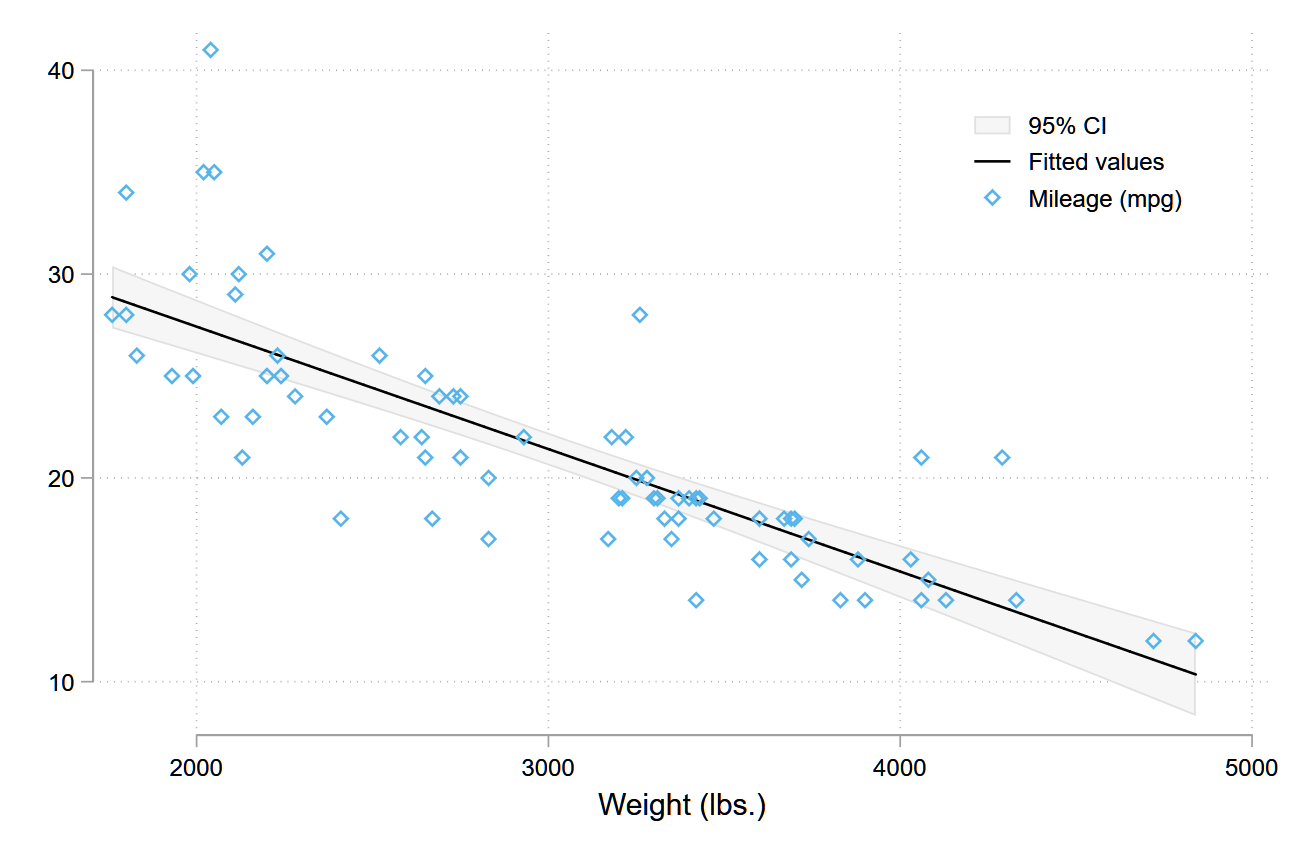
\includegraphics[width=0.6\textwidth]{mpg.png}
	\caption{MPG 和 Weight 的关系图\label{fig:mpg}}
\end{figure}



以最简单的一元线性模型来解释最小二乘法。什么是一元线性模型呢?监督学习中,如果预测的变量是离散的,我们称其为分类(如决策树,支持向量机等),如果预测的变量是连续的,我们称其为回归。回归分析中,如果只包括一个自变量和一个因变量,且二者的关系可用一条直线近似表示,这种回归分析称为一元线性回归分析。如果回归分析中包括两个或两个以上的自变量,且因变量和自变量之间是线性关系,则称为多元线性回归分析。对于二维空间线性是一条直线;对于三维空间线性是一个平面,对于多维空间线性是一个超平面。


\begin{property}
柯西列的性质
\begin{enumerate}[noitemsep]
\item $\{x_k\}$ 是柯西列,则其子列 $\{x_k^i\}$ 也是柯西列。
\item $x_k\in \mathcal{R}^n$,$\rho(x,y)$ 是欧几里得空间,则柯西列是收敛的,$(\mathcal{R}^n,\rho)$ 空间是完备的。
\end{enumerate}
\end{property}


\begin{conclusion}
回归分析(regression analysis) 是确定两种或两种以上变量间相互依赖的定量关系的一种统计分析方法。运用十分广泛,回归分析按照涉及的变量的多少,分为一元回归和多元回归分析;按照因变量的多少,可分为简单回归分析和多重回归分析;按照自变量和因变量之间的关系类型,可分为线性回归分析和非线性回归分析。如果在回归分析中,只包括一个自变量和一个因变量,且二者的关系可用一条直线近似表示,这种回归分析称为一元线性回归分析。如果回归分析中包括两个或两个以上的自变量,且自变量之间存在线性相关,则称为多重线性回归分析。
\end{conclusion}



\nocite{EINAV2010,Havrylchyk2018} 

\bibliographystyle{aer}
\bibliography{reference}

\appendix
\chapter{线性代数}

\section{矩阵的分块}

\begin{equation} 
\begin{vmatrix}
A_1 & 0\\
C & A_2
\end{vmatrix}
=|A_1|\times |A_2|
\end{equation}

由矩阵 $A$ 的若干行、若干列的交叉位置元素按照原来顺序排成的矩阵称为 $A$ 的一个\textbf{子矩阵}。

\end{document}
